% id: 0339
% book: RPM 중3-2 수학 · 03 원과 직선
% section: 중단원 마무리하기
% figure: crop:fig-0339.png
% answer: ③
% answer_source: 답지
% variant_level: 0 (원본 전사)
% 이 파일은 build.mjs 가 items.json 에서 만든다. 고칠 때는 items.json 을 고친다.
\noindent\begin{minipage}[t]{0.58\linewidth}\vspace{0pt}\raggedright 오른쪽 그림과 같이 반지름의 길이가 $10\mkern3mu \mathrm{cm}$인 원~$\pt{O}$에서 $\seg{AB}\parallel\seg{CD}$이고 $\seg{AB}=\seg{CD}=12\mkern3mu \mathrm{cm}$일 때, 두 현~$\pt{AB}$와 $\pt{CD}$ 사이의 거리는?\end{minipage}\hfill\begin{minipage}[t]{0.4\linewidth}\vspace{0pt}\centering \setlength{\dmfigw}{60.7pt}\ifdim\dmfigw>\linewidth\setlength{\dmfigw}{\linewidth}\fi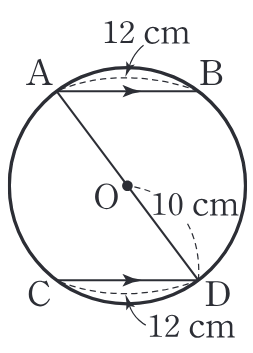
\includegraphics[width=\dmfigw]{figures/fig-0339.png}\end{minipage}\par
\begin{choicesii}{$14\mkern3mu \mathrm{cm}$}{$15\mkern3mu \mathrm{cm}$}{$16\mkern3mu \mathrm{cm}$}{$17\mkern3mu \mathrm{cm}$}{$18\mkern3mu \mathrm{cm}$}\end{choicesii}
